\chapter{Analysis of the Results and Discussion} \label{chap:results}

\section{Measurement of engagement ground truth}
The acquisition of the grand truth was performed by two different observers that were not into the interaction field, but with direct vision towards the subjects. A result of that visual assessment is shown in figure \ref{fig:GTexample}. The rest of the results are shown in the appendix \ref{appendix}.

\begin{figure}[h!]
        \centering
        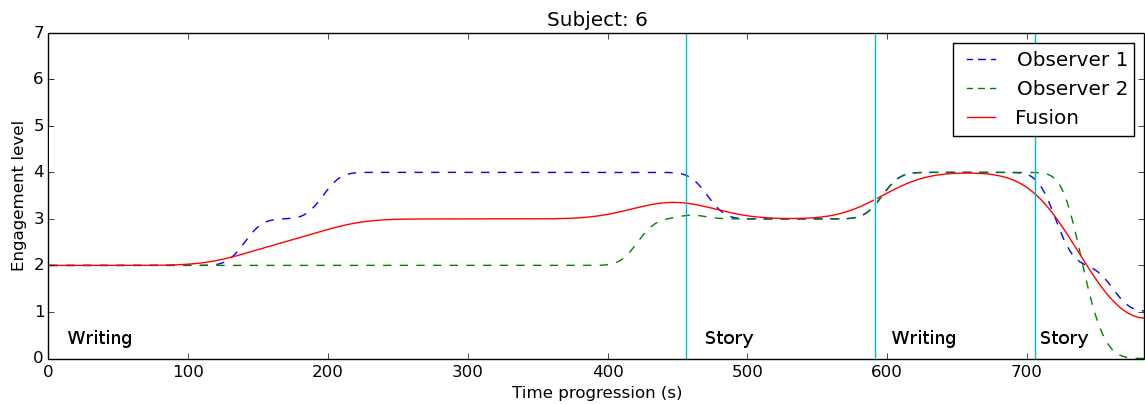
\includegraphics[width=0.6\textwidth]{figures/GTexample.png}
        \caption{Example of grand truth acquisition and fusion. The vertical lines indicate the story telling activity.}
        \label{fig:GTexample}
\end{figure}

It is important before comparing any result to check the inter rater reliability of the two observers, in another words, the inter-rater reliability for the ground truth. This measurement shows if the data can be used, or not, for that specific purpose of comparison and reference with respect to the feature measurements acquired. 

In order to do that, it is necessary to apply an arithmetic mean to the engagement value assessed by each of the observers taking into account each child in both CoWriter (writing) and story telling activities. Then, applying a Cronbach's alpha test (see equation \ref{eq:cronbach} in appendix), In this case, $\alpha = .82$ over the 6 subjects showing an agreement between both observers.

Furthermore, a one-way between groups ANOVA was run to see any relevance between the assessment measurement in both activities. In another words, if the measurements show enough variance to be used as ground truth. The result obtained was: $F[1,22] = 9.07 \quad p=.006$ (see appendix \ref{ap:GT}), which reveals that the activities lead to significantly different level of engagement.


\section{Movement and proximity across the two activities}
For quantity of movement (QoM) and proximity respectively, in both cases, greater means correspond to the writing activity as we can see in figures \ref{fig:meanMov} and \ref{fig:meanProx}. It leads to the assertion that the QoM and the proximity are directly related at least, with an active or passive activity.

Since the population studied does not exceed the 6 participants, we can not assume the data is normally distributed thus a T-test makes an estimation of the deviation instead of the real value considering a peer-wise comparison.

The results obtained from the T-test for both features shows a marginal significance in the QoM $ (t(df=10)= 2.0964, p = 0.06245) $ and significance \footnote{There is significance when $p<0.05$ and marginal significance when $p<0.1$} for the proximity measurement $(t(df=9.7406)= -2.8338, p = 0.01818) $. In addition, mean and standard deviation are shown in table \ref{tab:pvalues}.

\begin{figure}[h!]
        \centering
        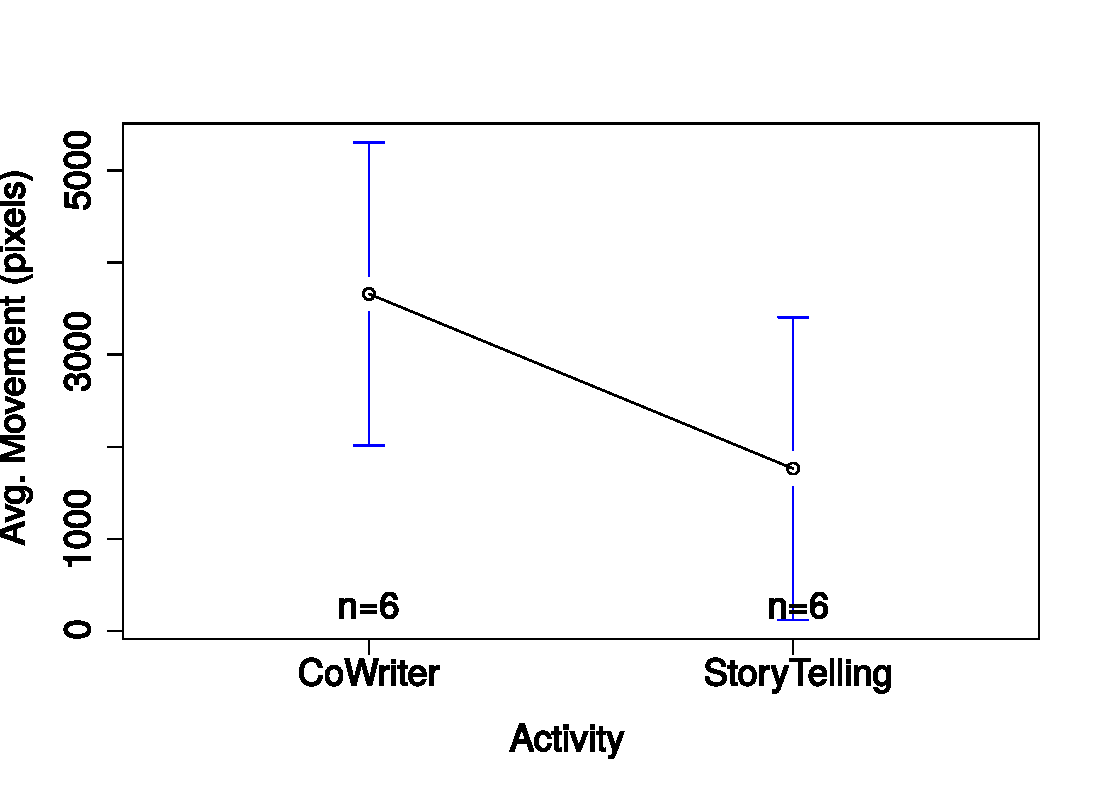
\includegraphics[width=0.7\textwidth]{figures/AvgMovement}
        \caption{QoM mean plot(ends show the confidence interval) across the two activities.}
		\label{fig:meanMov}
\end{figure}


\begin{figure}[h!]
        \centering
        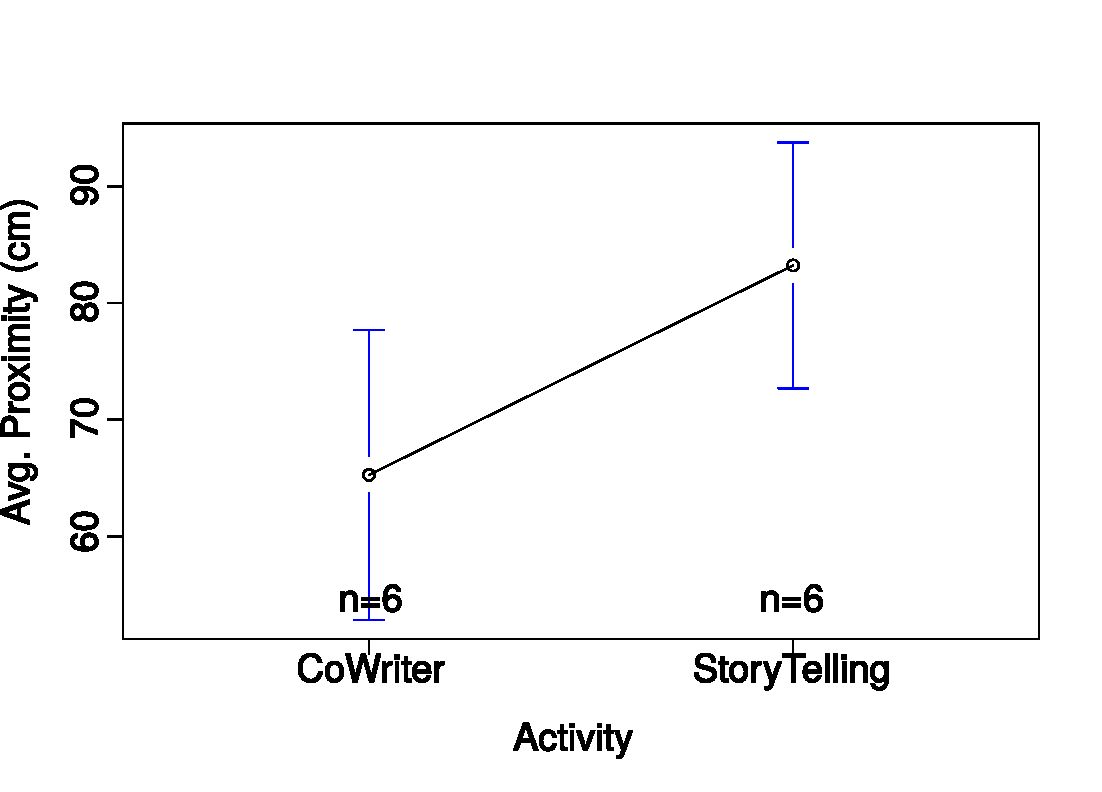
\includegraphics[width=0.7\textwidth]{figures/AvgProximity.pdf}
        \caption{Proximity mean plot(ends show the confidence interval) across the two activities.}
		\label{fig:meanProx}
\end{figure}


\begin{table}[h!]
\centering
\begin{tabular}{l|l|l|l|l}
          & \multicolumn{2}{c|}{\textbf{Writing}}                               & \multicolumn{2}{c|}{\textbf{Story telling}}                        \\ \cline{2-5} 
          & \multicolumn{1}{c|}{$\mu$} & \multicolumn{1}{c|}{$\sigma$} & \multicolumn{1}{c|}{$\mu$} & \multicolumn{1}{c}{$\sigma$} \\ \hline
\textbf{QoM}  &          3658.783                  &         1567.510                      &              1763.050              &              1564.938                \\ \hline
\textbf{Proximity} &      65.26000                      &           11.83703                    &          83.21667                  &              10.04000                
\end{tabular}
\caption{T-test mean, $\mu$ and standard deviation, $\sigma$ (see appendix \ref{ap:across}).}
\label{tab:pvalues}
\end{table}


However, a more accurate measurement across groups is performed by an ANOVA. In this case, a one way repeated measures ANOVA was used since we have a single group (6 subjects) on which we have measured the QoM and the proximity a few times (for writing and story telling activities) during the same amount of time. The results shown a significance \textit{F[1,115]=21.01, p=1.17e-05} being \textit{p<.001} for proximity and no significance for QoM \textit{F[1,286]=0.729, p=0.394}.

As we can see, the proximity measurement is significant. Therefore, the proximity to the interaction field is a good indicator of the child engagement in an active activity. In addition, the results are consistent with the lines shown in figures \ref{fig:anovaMov} and \ref{fig:anovaProx}, where in both cases the two groups are rather close together. However, relevant information can be extracted from the test output. The within subject test indicates that there is a significant relation between subjects, in other words, the groups do change between subjects but preserve a similar difference between activities. It shows that not all subjects share the same rank of movement and position.

\begin{figure}[h!]
        \centering
        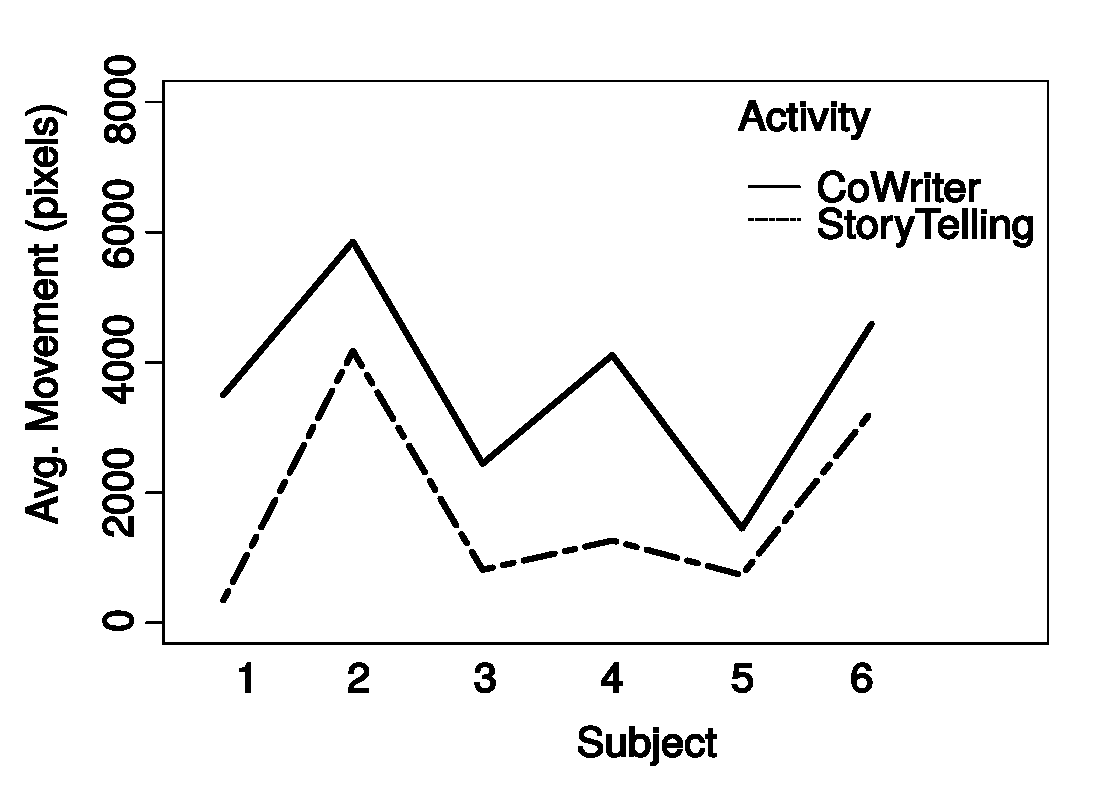
\includegraphics[width=0.7\textwidth]{figures/AvgMovement2.pdf}
        \caption{Inter-subject measurement variability for QoM.}
		\label{fig:anovaMov}
\end{figure}

\begin{figure}[h!]
        \centering
        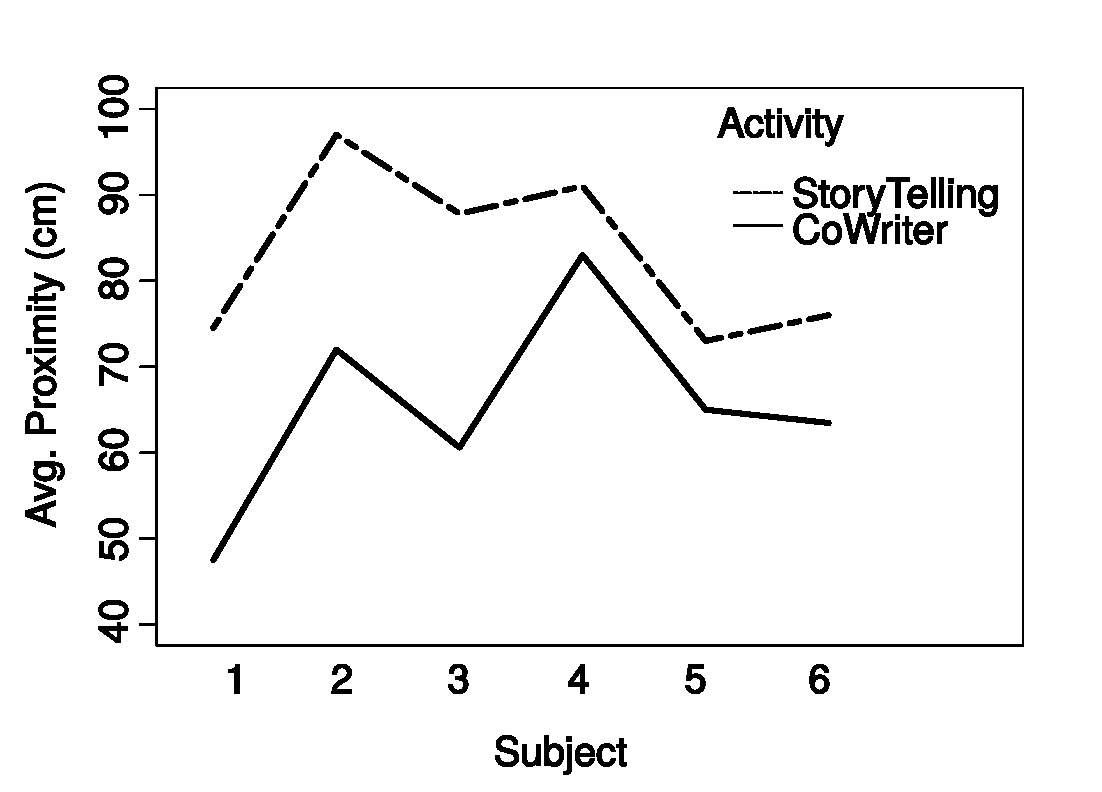
\includegraphics[width=0.7\textwidth]{figures/AvgProximity2.pdf}
        \caption{Inter-subject measurement variability for proximity.}
		\label{fig:anovaProx}
\end{figure}

It is necessary to say that these results need to be contrasted evaluating a greater number of subjects.
\\\\\\
Finally, in figure \ref{fig:avgProximity} we can see the average normalized proximity between the subjects over time, where the vertical lines indicate the story telling starting point in each case. In 5 over 6 subjects there is a tendency to decrease the proximity to the field of interaction right after the execution of the story telling activity.

\begin{figure}[h!]
        \centering
        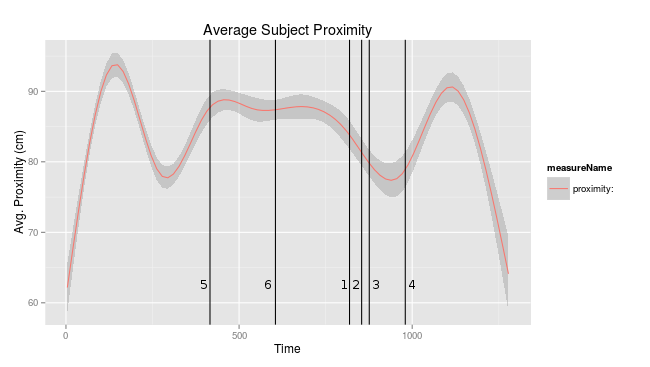
\includegraphics[width=1\textwidth]{figures/avgProximity.png}
        \caption{Average proximity measurement between subjects. The vertical lines indicate the start of the story telling activity.}
        \label{fig:avgProximity}
\end{figure}

\section{The gaze information}

After a preliminary analysis of the gaze direction, we noticed that in this specific context this feature does not provide a reliable measurement of engagement. However, it becomes interesting from the interaction point of view, being able to show the amount of intervention \ref{fig:gaze} needed from the facilitator sitting on the left of the subject, against the visual contact towards the field of interaction (robot and tablet).


 \begin{figure}[!htb]
	\centering
	\begin{tikzpicture}[>=latex]

		\node[inner sep=0pt] (xtion) at (0,0) {
		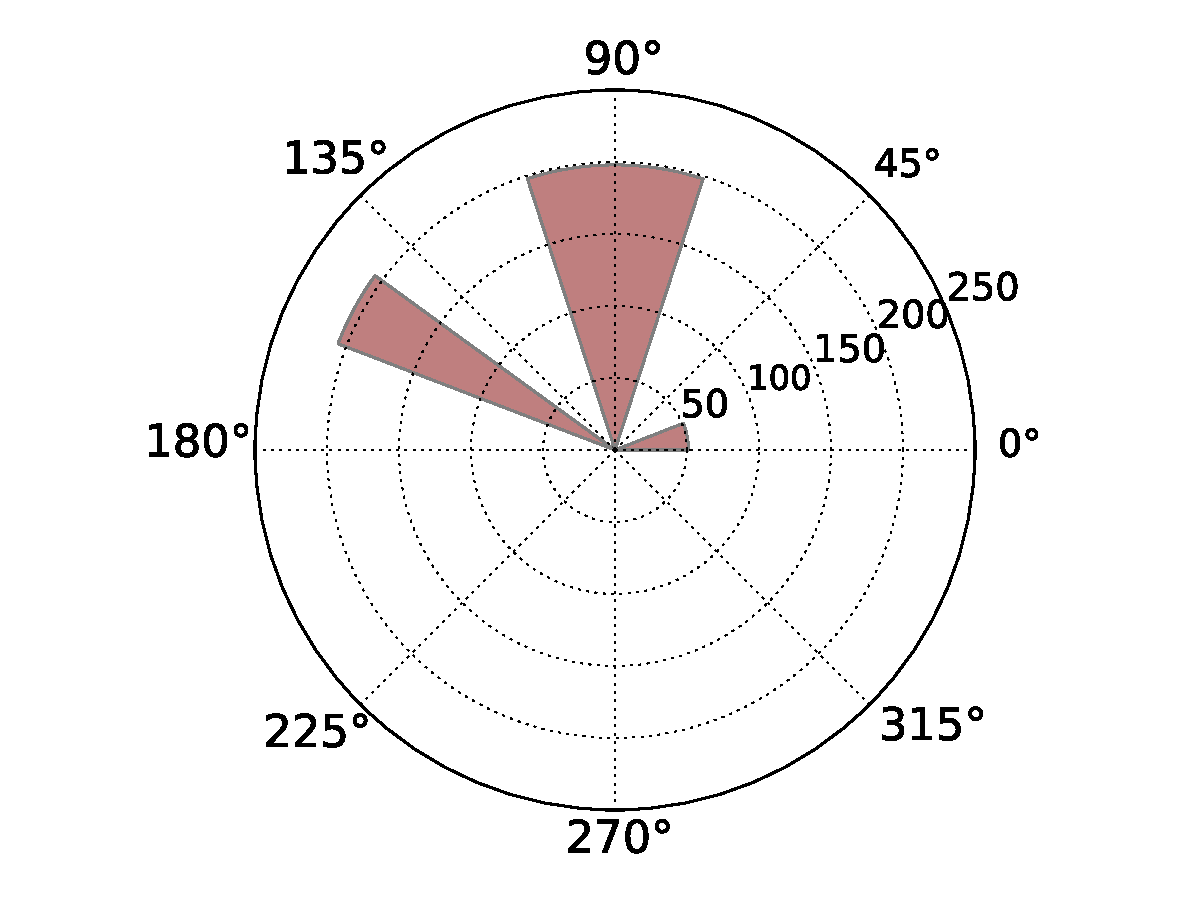
\includegraphics[width=0.6\textwidth]{figures/gaze.pdf}};
	
		\node[black, text width=2cm] at (0.74,1.8) {		
		Robot	
		};
		
		\node[black, text width=2cm] at (-1.3,0.5) {		
		Facilitator	
		};
				
	\end{tikzpicture}
    \caption{Subject's mean gaze direction being the $ 90\degree $ the robot and tablet together, and the range comprised between $ 135\degree-180\degree $ the location of the facilitator.}
    \label{fig:gaze}
\end{figure}

Using a range of age comprised in between 5-6 years old requires a high level of intervention. In this study, this accounts for almost half percent of the interaction time spend in front of the agent. Therefore, we can hypothesize that during the writing activity the children look more to the left and less to the robot in comparison with the story telling activity.

It is also important to test how likely it is that an observed distribution is due to chance or not using Pearson's Chi-squared (see equation \ref{eq:chi} in appendix). The result $(\chi^2(df=6,  N=537.75), p-value < 2.2e-16)$ shows a tiny chance. Secondly, in order to verify the hypothesis formulated previously based on one subject observation, we can use the residuals of the Chi-squared test comparing the observed data. The results are summarized in table \ref{tab:chi}.

\begin{table}[h!]
\centering
\begin{tabular}{l|l|l|l|l}
 		 		  & \textbf{Down} & \textbf{Left}	& \textbf{Right} & \textbf{Robot}	    \\ \hline	
 \textbf{Writing} &  102(3.4811216) & 2965(4.454916) & 35(-0.1499802)  &  993(-7.701501)    \\ \hline
 \textbf{Story telling}    &    0(-1.1542352) & 215(-10.687569)      & 6(0.3598100)      & 371(18.476290)
\end{tabular}
\caption{Chi-square test results (see appendix \ref{ap:across}).}
\end{table}\label{tab:chi}

As we hypothesize, the users tend to change their gaze direction towards the \textit{facilitator} located to left and to the tablet during the writing activity whereas the attention towards is acquired during the story telling activity. It suggests a future improvement towards a more independent system in the writing activity.

